\documentclass{../bredelebeamer}
\usepackage{multirow}
\usepackage{pdfpages}
\usepackage{braket,bigstrut}
\usepackage{palatino}
\usepackage{multicol,bigstrut}
\usepackage{listings}
\usepackage{tikz}
\usepackage{pgfplots}
\pgfplotsset{compat=1.17}
\usepackage{booktabs}
\usepackage{amsmath,amssymb,amsfonts,cancel,physics,siunitx}
\usetikzlibrary{positioning,shadows,backgrounds,calc}%
\setbeamercolor{footnote mark}{fg=black}
\setbeamercolor{footnote}{fg=black}
\usepackage{appendixnumberbeamer}


\renewcommand{\baselinestretch}{0.9}

\usepackage[backend=bibtex8,style=authortitle,autocite=footnote]{biblatex}
\addbibresource{referencia.bib}

\renewbibmacro*{cite:title}{%
	\printtext[bibhyperref]{%
		\printfield[citetitle]{labeltitle}%
		\setunit{\space}%
		\printtext[parens]{\printdate}%
	}%
}
\renewcommand{\figurename}{{\bf Fig.}}
\usefonttheme{serif} % default family is serif

% Define arXiv command for stylized formatting
\newcommand{\arxiv}{ar$\chi$iv:}

\renewcommand{\baselinestretch}{0.9}

\title[Final Dissertation]{Machine Learning-Enhanced Feasibility Studies on the Production of New Particles with Preferential Couplings to Third Generation Fermions at the LHC}
\subtitle{}
\author[ML-BSM3G@LHC - C. Rodríguez]{%
    \vspace{2em}\\
    PhD(c). Cristian Fernando Rodríguez Cruz\inst{1}\\
    \href{mailto:c.rodriguez45@uniandes.edu.co}{c.rodriguez45@uniandes.edu.co}\\
    \vspace{1em}
    Research advisors:\\
    \vspace{0.5em}
    Prof. Andrés Florez\inst{1} ( \href{mailto:ca.florez@uniandes.edu.co}{ca.florez@uniandes.edu.co} )\\
    \vspace{0.5em}
    Prof. J. Jones-Pérez\inst{2} ( \href{mailto:jones.j@pucp.edu.pe}{jones.j@pucp.edu.pe} )\\
    \vspace{1em}
}

\institute[]{\inst{1} Universidad de los Andes\and
\inst{2} Pontificia Universidad Católica del Perú
}
\date{\today}
\lstset{language=C++,
  basicstyle=\ttfamily,
  keywordstyle=\color{blue}\ttfamily,
  stringstyle=\color{red}\ttfamily,
  commentstyle=\color{green}\ttfamily,
  morecomment=[l][\color{magenta}]{\#}
}

\newcounter{finalframe}

% Flag to control section divider frames
\newif\ifsectiondividers
\sectiondividersfalse  % Set to false to hide divider frames
\sectiondividerstrue   


\begin{document}
\frame{\titlepage}

\begin{frame}
    \frametitle{Outline}
    \tableofcontents
\end{frame}

\section{Introduction}

\ifsectiondividers
\begin{frame}
\centering
\vfill
{\Huge \textbf{Introduction}}
\vfill
\end{frame}
\fi

\subsection{Standar Model of Particle Physics}
\begin{frame}
    
\end{frame}
\subsection{Deficiencies of the SM}
\begin{frame}

\end{frame}

\subsection{LHC and Beyond the SM Physics}
\begin{frame}

\end{frame}

\begin{frame}{The Quark-Gluon Sea}
	\begin{center}
		\includegraphics[width=0.95\textwidth]{../Images/pp_collision.png}
	\end{center}
\end{frame}

\section{Phenomenological Framework}

\ifsectiondividers
\begin{frame}
\centering
\vfill
{\Huge \textbf{Phenomenological Framework}}
\vfill
\end{frame}
\fi

\subsection{Madgraph-Pythia-Delphes}
\begin{frame}

\end{frame}

\subsection{Hypothesis Testing and Significance}
\begin{frame}

\end{frame}

\subsection{Machine Learning in High Energy Physics}
\begin{frame}

\end{frame}

\section{$U(1)_{T^3_R}$ Model}

\ifsectiondividers
\begin{frame}
\centering
\vfill
{\Huge \textbf{$U(1)_{T^3_R}$ Model}}
\vfill
\end{frame}
\fi
\subsection{}


\subsection{Production Channel}

\begin{frame}
	To do ADD production channel diagrams
\end{frame}
\begin{frame}{Feasible Experimental Signatures}{Cross Section}
	\begin{figure}
		\centering
		\includegraphics[width=.7\linewidth]{../Images/cross_section_by_masses.pdf}
		\caption{Projected cross section (fb) plot for $pp\to t \chi_\mathrm{u} \phi'$ and subsequent decay as a function of $m(\chi_\mathrm{u})$ and $m(\phi')$.}
		\label{fig:xs-plot}
	\end{figure}
\end{frame}

\subsection{Search Channel}
\begin{frame}{Feasible Experimental Signatures}{Search Channel}
	Representative Feynman diagram for the production of a $\phi'$ boson in association with a $\chi_\mathrm{u}$ vector-like quark through the fusion of a top quark and $\chi_\mathrm{u}$ vector-like quark. 
	\begin{center}
		\includegraphics[width=0.5\textwidth]{../Images/main_channel.png}
	\end{center}
	The $\phi'$ decays to a pair of muons, the top quark decays fully hadronically, and the $\chi_\mathrm{u}$ decays semi-leptonically to muons, neutrinos and $b$-jets.
\end{frame}
\begin{frame}{Feasible Experimental Signatures}{Search Channel}
	Representative Feynman diagram for the production of a $\phi'$ boson in association with a $\chi_\mathrm{u}$ vector-like quark through the fusion of a gluon pair from incoming protons.
	\begin{center}
		\includegraphics[width=0.6\textwidth]{../Images/signal_ggfusion.pdf}
	\end{center}
	The $\phi'$ decays to a pair of muons, the top quark that decays fully hadronically, and the $\chi_\mathrm{u}$ decay semi-leptonically to muons, neutrinos and jets.
\end{frame}

\begin{frame}{Feasible Experimental Signatures}{Background}
	Representative Feynman diagram for a background event. A $Z$ boson is produced in association with a top quark through the fusion of a top, anti top pair from incoming protons. 
	\begin{center}
		\includegraphics[width=0.45\textwidth]{../Images/bg_Z_full.pdf}
	\end{center}
	The $Z$ boson subsequently decays to a pair of muons and the two spectator top quarks decay semi-leptonically and purely hadronically to muons, neutrinos and jets, resulting in the same final states as the signal event.
\end{frame}

\subsection{Kinematic Variables}

\begin{frame}{Feasible Experimental Signatures}{Kinematic Variables}
	\begin{figure}
	\centering
	\includegraphics[width=.6\linewidth]{../Images/PT_b1.pdf}
	\caption{Transverse momentum distribution of the leading \textrm{b}-quark jet candidate. The distributions are shown for the two main SM background processes and two signal benchmark points.\label{fig:pTb1}}
	\end{figure}
\end{frame}

\begin{frame}{Feasible Experimental Signatures}{Kinematic Variables}
	\begin{figure}
	\centering
	\includegraphics[width=.6\linewidth]{../Images/PT_mu1_1.pdf}
	\caption{Transverse momentum distribution of the leading muon candidate. The distributions are shown for the two main SM background processes and two signal benchmark points.\label{fig:pTmu1}}
	\end{figure}
\end{frame}

\begin{frame}{Feasible Experimental Signatures}{Kinematic Variables}
	\begin{figure}
	\centering
	\includegraphics[width=.6\linewidth]{../Images/M_mu_1_2.pdf}
	\caption{Invariant mass distribution of the muon pair with the highest and second highest transverse momentum. The distributions are shown for the two main SM background processes and two signal benchmark points.\label{fig:_mu12}}
	\end{figure}
\end{frame}

\subsection{Gradient Boosting}
\begin{frame}{Feasible Experimental Signatures}{Gradient Boosting}
	\begin{figure}
		\centering
		\includegraphics[width=.6\linewidth]{../Images/feature_importance.pdf}
		\caption{Relative importance of features in training for a benchmark signal scenario with $m(\phi')=325\, \mathrm{GeV}$ and $m(\chi_\mathrm{u})=2000\, \mathrm{GeV}$.}
		\label{fig:feature_importance}
	\end{figure}
\end{frame}

\begin{frame}{Feasible Experimental Signatures}{Gradient Boosting}
	\begin{figure}
	\centering
		\centering  \includegraphics[width=.6\linewidth]{../Images/XGB_output.pdf}
		\caption{Output of the gradient boosting algorithm for a benchmark $m(\phi') = 100$~\textrm{GeV} and $m(\chi_\mathrm{u}) = 500\, \mathrm{GeV}$ signal, and dominant backgrounds. The distributions are normalized to unity.}
		\label{fig:xgboostout}
	\end{figure}
\end{frame}

\begin{frame}{Signal Significance}
	\begin{figure}[]
		\centering
		\includegraphics[width=.8\linewidth]{../Images/significance.pdf}
		\caption{Signal significance for the high luminosity LHC era, considering with 3000  $\mathrm{fb}^{-1}$ of collected data.}
		\label{fig:/significance_3000}
	\end{figure}
\end{frame}


\section{$U_1$ Leptoquark Model}

\ifsectiondividers
\begin{frame}
\centering
\vfill
{\Huge \textbf{$U_1$ Leptoquark Model}}
\vfill
\end{frame}
\fi

\begin{frame}{The vector leptoquark $U_1$ model}
	\begin{multicols}{2}
	A leptoquark is defined as a particle with a vertex that mix vectors and quarks.
	\begin{center}
	\includegraphics[width=.25\textwidth]{../Images/LQ_vertex.png}
	\end{center}
	If $U_1$ is a vector leptoquark that preserves the chirality on the vertex, we expect an interaction term like
	$$
	\sim \beta_L U_1^\mu\bar{q}_{L} \gamma_{\mu} \ell_{L},
	$$
	and these allows a similar interaction term for the right handed currents 
	$$
	\sim \beta_R U_1^\mu\bar{d}_{R} \gamma_{\mu} e_{R}.
	$$

	\end{multicols}
    %$$ $$
	\begin{minipage}{.32\linewidth}
		\centering
		\includegraphics[width=\linewidth]{../Images/non_resonant.png}\\
		Non-resonant
	\end{minipage}\hfill
	\begin{minipage}{.32\linewidth}
		\centering
		\includegraphics[width=\linewidth]{../Images/single_LQ.png}\\
		Single LQ
	\end{minipage}\hfill
	\begin{minipage}{.32\linewidth}
		\centering
		\includegraphics[width=\linewidth]{../Images/double_LQ.png}\\
		Double LQ
	\end{minipage}
\end{frame}

\begin{frame}{Leptoquark Production at pp Colliders}
    \includegraphics[width=.48\textwidth]{../Images/BR.png}
    \raisebox{-1.0em}{\includegraphics[width=.51\textwidth]{../Images/XS.png}}
\end{frame}

\subsection{Kinematic Feature Eng.}
\begin{frame}{$S_T^{\text{meT}}=\text{met} + \sum_i\left|p_{T}^i\right|$}
	\begin{center}
		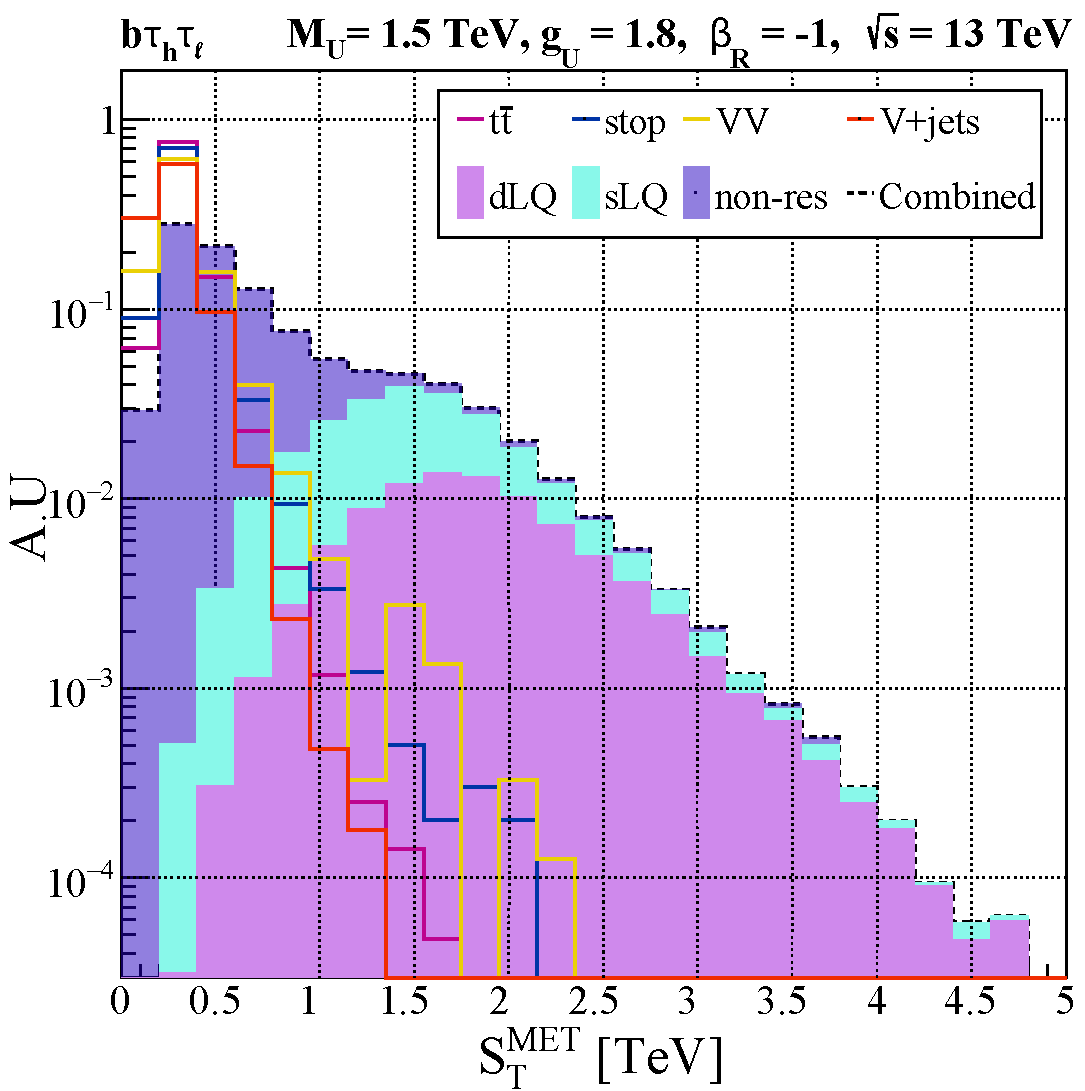
\includegraphics[width=.65\linewidth]{../Images/sTTeV_semileptonic_sLQ_wRHC.pdf}
	\end{center}
	
\end{frame}

\begin{frame}{$\Delta R = \sqrt{\Delta \eta^2 + \Delta \phi^2}$}
	\begin{center}
		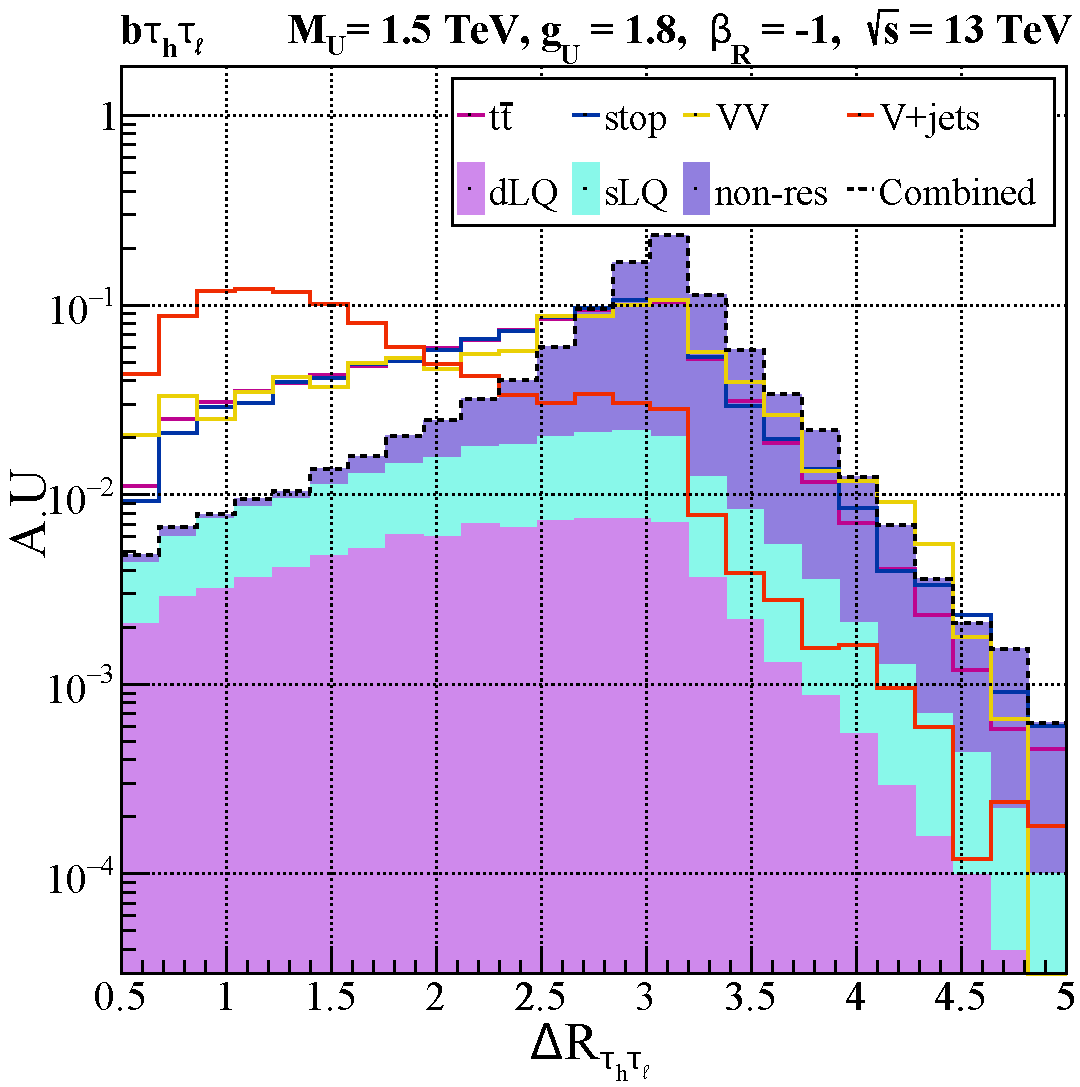
\includegraphics[width=.65\linewidth]{../Images/DeltaR_semileptonic_sLQ_wRHC.pdf}	
	\end{center}
	
\end{frame}

\begin{frame}{The optimized observable}{XGB-output}

	We can evaluate a score for the signal and background events using the discriminator algorithm. 

	\begin{center}
		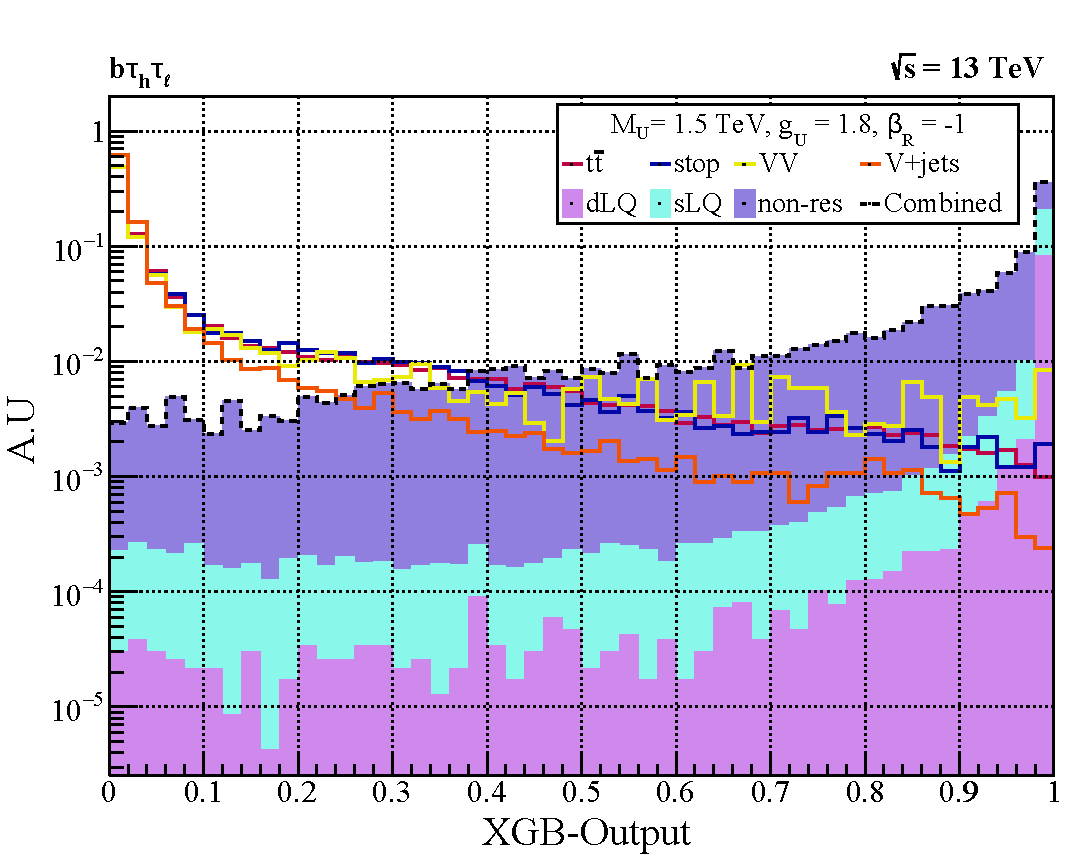
\includegraphics[width=.75\linewidth]{../Images/ML_semileptonic_sLQ_wRHC.pdf}
	\end{center}
		
\end{frame}

\subsection{Single Channels Sensitivity Reach}

\begin{frame}{Double Leptoquark Production}{The Sensitivity Reach / only left-handed currents}
	\begin{minipage}{.30\linewidth}
		\includegraphics[width=\linewidth]{../Images/double_LQ.png}
	\end{minipage}
	\begin{minipage}{.68\linewidth}
		\includegraphics[width=\linewidth]{../Images/Significance_Heatmap_13TeV_L137_dLQ_combined_woRHC.pdf}
	\end{minipage}
	{\large
	  Double leptoquark production is sensitive to the leptoquark mass, its production depends only on the QCD coupling constant and the available energy.
	}
\end{frame}

\begin{frame}{Single leptoquark production}{The Sensitivity Reach / only left-handed currents}
	\begin{minipage}{.30\linewidth}
		\includegraphics[width=\linewidth]{../Images/single_LQ.png}
	\end{minipage}
	\begin{minipage}{.68\linewidth}
		\includegraphics[width=\linewidth]{../Images/Significance_Heatmap_13TeV_L137_sLQ_combined_woRHC.pdf}
	\end{minipage}
	{\large
		  Single leptoquark production is sensitive to both, mass and couplings. It contributes to the regions of high coupling constants at higher masses than double leptoquark production.
	}
\end{frame}

\begin{frame}{Non-resonant Production}{The Sensitivity Reach / only left-handed currents}
	\begin{minipage}{.30\linewidth}
		\includegraphics[width=\linewidth]{../Images/non_resonant.png}
	\end{minipage}
	\begin{minipage}{.68\linewidth}
		\includegraphics[width=\linewidth]{../Images/Significance_Heatmap_13TeV_L137_non-res_combined_woRHC.pdf}
	\end{minipage}

	{\large
		  Non-resonant production is highly dependent on the couplings, so it dominates the regions of high coupling constants at all masses.
	}
\end{frame}

\subsection{Combined Sensitivity Reach}
\begin{frame}{Combined Sensitivity Reach}{The Sensitivity Reach / only left-handed currents}
	\begin{center}
		\includegraphics[width=.41\linewidth]{../Images/Significance_Curves_13TeV_L137_summary_all_sigmas_woRHC.pdf}
		\pause
		\includegraphics[width=.55\linewidth]{../Images/Significance_Heatmap_13TeV_L137_all_combined_woRHC.pdf}
	\end{center}
	{\large
		The sensitivity of
		all signal production processes combined compares
		our expected exclusion region with the latest one from
		the ATLAS Collaboration [ArXiv:2305.15962], but we suggest better sensitivity for high coupling constants.
	}
	
\end{frame}

\begin{frame}{Combined Sensitivity Reach}{The Sensitivity Reach / only right-handed currents}
	\begin{center}
		\includegraphics[width=.7\linewidth]{../Images/Significance_CMS_Comparison_13TeV_L137_all_combined_woRHC.pdf}
	\end{center}
	{\large
		  The case $BR(lq \rightarrow b \tau) = 1$ corresponds to the only right-handed currents coupling. The sensitivity compared with the latest one from the CMS [2308.07826] and ATLAS Collaborations [2303.01294], again we suggest better sensitivity for high coupling constants.
	}
\end{frame}


\section{$Z'$ Interferences}

\ifsectiondividers
\begin{frame}
\centering
\vfill
{\Huge \textbf{$Z'$ Interferences}}
\vfill
\end{frame}
\fi

\begin{frame}{The need of a $Z'$ boson in gauge $U_1$ models}
    If $U_1$ has a gauge origin,  we could rewrite the interaction term in the covariant derivative as
	$$
	\psi_{L}^{\mathrm{SM}}=\begin{pmatrix}
		q_{Lr}\\ q_{Lg}\\ q_{Lb}\\ \ell_L
	\end{pmatrix}
	\Longrightarrow\;\;
	\mathcal{L}_{\text{int}}
	\sim U_{1\alpha}^\mu \bar{\psi}_{L}^{\mathrm{SM}}\, \gamma_{\mu} T_{+}^{\alpha } \psi_{L}^{\mathrm{SM}} + \text{h.c.},
	\quad
	T_{+}^{\alpha}=\begin{pmatrix}
		0 & 0 & 0 & \delta_{r\alpha}\\
		0 & 0 & 0 & \delta_{g\alpha}\\
		0 & 0 & 0 & \delta_{b\alpha}\\
		0 & 0 & 0 & 0
	\end{pmatrix},
	$$
	we have six generators $T_{\pm}^{\alpha }$ with closure relation and projecting into a color singlet operator:
	$$
	\sum_{\alpha} \left[{T_{+}^{\alpha }},{T_{-}^{\alpha}}\right] =
	3 T_{B-L}=\begin{pmatrix}
		1 & 0 & 0 & 0\\
		0 & 1 & 0 & 0\\
		0 & 0 & 1 & 0\\
		0 & 0 & 0 & -3
	\end{pmatrix}.
	$$
	So, the gauge group with this leptoquark must include a $U(1)_{B-L}$ symmetry (The right-handed currents also have a similar interaction term).
    
    \pause
    $$ $$
    The interaction terms for the $Z'$ boson have the form
	\begin{align*}
		\mathcal{L}_{\text{int}} &\sim Z'_\mu\left(\bar{\psi}_{L}^{\mathrm{SM}}\gamma^\mu (3T_{B-L}) \psi_{L}^{\mathrm{SM}}\right)\\
		&\sim Z'_\mu \left(\bar q_{L} \gamma^\mu q_{L} - 3 \bar \ell_L \gamma^\mu \ell_L\right).
	\end{align*}
\end{frame}
\begin{frame}{Interference with a $Z'$ vector boson}
\begin{minipage}{.48\linewidth}
	Non-Resonant Production (leptoquarks)
	\begin{center}
		\includegraphics[width=.9\linewidth,height=.5\linewidth]{../Images/non-res_vector.pdf}
	\end{center}
	\begin{equation}
		\mathcal{M}_{U_1} \sim \frac{1}{t-m_{U_1}^2 + i m_{U_1} \Gamma_{U_1}},
	\end{equation}
\end{minipage}
\hfill
\begin{minipage}{.48\linewidth}
	Resonant Production (neutral bosons)
	\begin{center}
		\includegraphics[width=.9\linewidth,height=.5\linewidth]{../Images/DY.pdf}
	\end{center}
	\begin{equation}
		\mathcal{M}_{Z'} \sim \frac{1}{s-m_{Z'}^2 + i m_{Z'} \Gamma_{Z'}},
	\end{equation}
\end{minipage}
so the interference has the form
	\begin{equation*}
		% \mathrm{RKI}
		% 			=\frac{1}{\sigma_{ LQ+Z'}}
					\dv{m}\left[
							\sigma_{ LQ+Z'}-\left(\sigma_{ LQ} +\sigma_{Z'}
							\vphantom{\frac{1}2}
							\right)
							\right]
							\sim \frac{g_{z'}g_{U}}{s}\frac{ m_{LQ}m_{Z'}\Gamma_{LQ}\Gamma_{Z'} - (t-m_{LQ}^2)(s-m_{Z'}^2)}{\left[
					(t-m_{LQ}^2)^2 + m_{LQ}^2\Gamma_{LQ}^2
			\right]
			\left[
					(s-m_{Z'}^2)^2 + m_{Z'}^2\Gamma_{Z'}^2
			\right]}.
	\end{equation*}

    Similary for Polarized final states.
\end{frame}

\begin{frame}{Interference with a $Z'$ vector boson}


	\begin{center}
		\includegraphics[width=.45\linewidth]{../Images/Kinematic_Interference_gu_1.0_gzp_1.0_zp_upper_limit_woRHC.pdf}
		\hfill
		\includegraphics[width=.53\linewidth]{../Images/xs_interference.png}
	\end{center}
\end{frame}

\begin{frame}{Effects on the Sensitivity reach}
	
	\begin{center}
		\includegraphics[width=.48\linewidth]{../Images/reach_wo_interference.png}
		\hfill
		\includegraphics[width=.48\linewidth]{../Images/reach_w_interference.png}
	\end{center}
	
\end{frame}

\section{Summary and Conclusions}

\ifsectiondividers
\begin{frame}
\centering
\vfill
{\Huge \textbf{Summary and Conclusions}}
\vfill
\end{frame}
\fi

\begin{frame}

\end{frame}

%ADD a slide marker for backlog frames
\ifsectiondividers
	\begin{frame}
		\centering
		\vfill
		{\Huge \textbf{Backup Slides}}
		\vfill
	\end{frame}
\fi
\appendix

\section{Formalism of the gauge $U_1$ leptoquark}
\begin{frame}%{Formalism of the gauge $U_1$ leptoquark}
    Where the SM charges for the leptoquark, in the $Y=2(Q-T_3)$ convention, are
	\begin{center}
		\begin{tabular}{|c|c|c|c|c|}
			\hline & $\bar{q}_{L}$ & $\ell_{L}^{j}$ & $\bar{q}_{L}\gamma_{\mu} \ell_{L}$ & $U_{1}^{\mu}$ \\
			\hline$U(1)$ & $-1 / 3$ & $-1 $ & $-4 / 3$ & $+4 / 3$ \\
			\hline $\mathrm{SU}(2)$ & $\overline{\mathbf 2}$ & $\mathbf{2}$ & $\mathbf{1}$ & $\mathbf{1}$ \\
			\hline $\mathrm{SU}(3)$ & $\overline{\mathbf 3}$ & $\mathbf{1}$ & $\overline{\mathbf3}$ & $\mathbf{3}$ \\
			\hline
		\end{tabular}	
	\end{center}
	Then, the leptoquark $U_1 \sim \left(\mathbf{3}_{C}, \mathbf{1}_{I}, 4 / 3_{Y}\right)$. 

    \pause
    $$ $$
    The full Lagrangian for the vector leptoquark is
	\begin{align*}
		\mathcal{L}_{U}=&-\frac{1}{2} U_{\mu \nu}^{\dagger} U^{\mu \nu}+M_{U}^{2} U_{\mu}^{\dagger} U^{\mu}-i g_{s}U_{\mu}^{\dagger} T^{a} U_{\nu} G^{\mu \nu}_a -\frac{2 i}{3} g' U_{\mu}^{\dagger} U_{\nu} B^{\mu \nu}\\
		&+\frac{g_{U}}{\sqrt{2}}\left[U_{1}^{\mu}\left(\beta_{L}^{i j} \bar{q}_{L}^{i} \gamma_{\mu} e_{L}^{j}+\beta_{R}^{i j} \bar{d}_{R}^{i} \gamma_{\mu} e_{R}^{j}
		%+\beta_{N}^{i} \bar{u}_{R}^{i} \gamma_{\mu} N_{R}
		\right)+\text { h.c. }\right]
	\end{align*}
	where $U_{\mu \nu}=\mathcal D_{\mu} U_{\nu}-\mathcal D_{\nu} U_{\mu}$, $\mathcal D_{\mu}=\partial_{\mu}-i g_{s} G_{\mu}^{a} T^{a}-i \frac{2}{3} g_{Y} B_{\mu}$, and the couplings $\beta_{L}$ and $\beta_{R}$ are complex $3 \times 3$ matrices in flavor space. 

    \pause 
    $$ $$
    Constraints from $\Delta F=2$ and lepton flavor violation impose a hierarchy with dominant third generation couplings: 
    
    \begin{equation}
     \left|\beta_L^{11}\right|, \left|\beta_L^{12}\right|, \left|\beta_L^{21}\right|, \left|\beta_L^{22}\right|, \left|\beta_L^{31}\right| \ll \left|\beta_L^{13}\right| \ll\left|\beta_L^{23}\right|,\left|\beta_L^{32}\right| \ll\left|\beta_R^{33}\right|,\left|\beta_L^{33}\right|=\mathcal{O}(1)   ,
    \end{equation}
    where $\beta_R$ is diagonal.
\end{frame}

\section*{Two body scattering}
\begin{frame}{Two body scattering}{CM-Frame}
    Consider the process
    \begin{equation}
        A(\va*{p}_1) + B(\va*{p}_2) \longrightarrow C(\va*{p}_3) + D(\va*{p}_4),
    \end{equation}
    \begin{center}
        \includegraphics[width=0.6\textwidth]{../Images/scatter.png}
    \end{center}

    From the Golden Rule, the cross section is given by
    \begin{equation}
        \sigma = \frac{n! (2\pi)^4}{4\sqrt{(\va*{p}_1\cdot\va*{p}_2)^2 - (m_1m_2)^2}}\int \abs{\mathcal{M}}^2\delta^{(4)}(p_1 + p_2 - p_3 - p_4)\frac{d^3\va*{p}_3}{(2\pi)^3 2E_3}\frac{d^3\va*{p}_4}{(2\pi)^3 2E_4}.
    \end{equation}
    But, in the CM frame, $\va*{p}_1 + \va*{p}_2 = 0$, where
    \begin{gather}
        \sqrt{(\va*{p}_1\cdot\va*{p}_2)^2 - (m_1m_2)^2} = E_1E_2 \abs{\va*{p}_1},
        \\
        \delta^{(4)}(p_1 + p_2 - p_3 - p_4) = \delta\left(
        E_1 + E_2 - E_3 - E_4
        \right)
        \delta^{(3)}(\va*{p}_3 + \va*{p}_4).
    \end{gather}
    Thus
    \begin{equation}
        \sigma = \left(\frac{1}{8\pi}\right)^2 \frac{n!}{(E_1E_2) \abs{\va*{p}_1}}\int \abs{\mathcal{M}}^2
        \frac{\delta\left(
            E_1 + E_2 - \sqrt{\va p_3^2 + m_3^2} - \sqrt{\va p_3^2 + m_4^2}
            \right)}{\sqrt{\va p_3^2 + m_3^2}\sqrt{\va p_3^2 + m_4^2}} \dd \va p_3
    \end{equation}
\end{frame}

\begin{frame}%{Two body scattering}{CM-Frame}
    Integrating over the radial part $\abs{\va p_3}$, we get
    \begin{equation}
        \sigma = \left(\frac{1}{8\pi}\right)^2 \frac{n! |\va*{p}_3|}{(E_1 +E_2)^2 \abs{\va*{p}_1}} \int \abs{\mathcal{M}}^2 \dd\Omega,
    \end{equation}
    with
    \begin{equation}
        |\va*{p}_3| = \frac{1}{2} \frac{\sqrt{((E_1+E_2)^2 - m_3^2 -m_4^2)^2- 4m^2_3m^2_4} }{E_1+E_2},
    \end{equation}
    the outgoing momentum in the CM frame.

    $$ $$

    We prefer work with differential cross section as
    \begin{equation}
        \frac{\dd \sigma}{\dd \Omega} = \frac{1}{64\pi^2} \frac{n! }{(E_1 +E_2)^2 } \frac{|\va*{p}_3|}{\abs{\va*{p}_1}} \abs{\mathcal{M}}^2.
    \end{equation}

    Defining $\sqrt s = E_1 + E_2$, we have
    \begin{equation}
        |\va*{p}_3| = \frac{1}{2} \frac{\sqrt{(s - m_3^2 -m_4^2)^2- 4m^2_3m^2_4} }{\sqrt s}, \quad  |\va*{p}_1|=\frac{1}{2} \frac{\sqrt{(s - m_1^2 -m_2^2)^2- 4m^2_1m^2_2} }{\sqrt s}.
    \end{equation}
    so the differential cross section is
    \begin{equation}
        \frac{\dd \sigma}{\dd \Omega} = \frac{1}{64\pi^2} \frac{n! }{s }
        \sqrt{\frac{(s - (m_3 + m_4)^2)(s - (m_3 - m_4)^2)}{(s - (m_1 + m_2)^2)(s - (m_1 - m_2)^2)}}
        \abs{\mathcal{M}}^2.
    \end{equation}

    Note that at this point, we don't need to know the explicit form of the matrix element $\mathcal{M}$, so it is a generic result.
\end{frame}

\begin{frame}{Writting $t$ in terms of $s$ and $\theta$}
    

    In general, there are three Lorentz-invariant useful kinematical variables to describe the scattering process, known as Mandelstam variables:
    \begin{align}
        \hat s & = (p_1 + p_2)^2 = (p_3 + p_4)^2 = m_1^2 + m_2^2 + 2p_1^\mu p_{2\mu }= m_3^2 + m_4^2 + 2p_3^\mu p_{4\mu}, \\
        \hat t & = (p_1 - p_3)^2 = (p_2 - p_4)^2= m_1^2 + m_3^2 - 2p_1^\mu p_{3\mu }= m_2^2 + m_4^2 - 2p_2^\mu p_{4\mu},  \\
        \hat u & = (p_1 - p_4)^2 = (p_2 - p_3)^2= m_1^2 + m_4^2 - 2p_1^\mu p_{4\mu }= m_2^2 + m_3^2 - 2p_2^\mu p_{3\mu}.
    \end{align}
    $$ $$
    In the CM-frame, $\hat s = s = (E_1+E_2)^2$. If, $m_3=m_4$ and $m_1=m_2$ with $E_1=E_2=E_3=E_4=E$, we have
    \begin{equation}
        t = -\left(\va p_1 - \va p_3\right)^2 = - \va p_1^2 - \va p_3^2 + 2\va p_1\va p_3 
    \end{equation}
    where $\va p_1^2 = E^2 - m_1^2 $  and $\va p_3^2 = E^2 - m_3^2 $.
    $$ $$
    So, in terms of $s$, $t$ could be written as
    \begin{equation}
        t= -2s + (m_1^2 + m_3^2) + 2\sqrt{(s/4 - m_1^2)(s/4 - m_3^2)} \cos\theta,
    \end{equation}
    with $\theta$ the scattering angle in the CM-frame.
\end{frame}



\end{document}
